% CAP description for Tree --> Expand by Textpath --> Textpath
\begin{itemize}
\item Use this parameter to specify the textpath of the subtree you want to expand.
\item Make sure you give the whole path (start from the very top of the tree).
\item Use slash {\tt '/'} as a path separator (to separate parent nodes from child nodes). 
\item Give the path to the node which you want to expand.
\item Each segment of the path will be used to find a corresponding node, using the Operator provided.
\end{itemize}

\textbf{Example:}

\begin{itemize}
\item Your tree looks like this:

\begin{figure}
\begin{center}
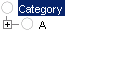
\includegraphics{PS/Treeexample3}
\caption{Tree 3}
\label{treeexample3}
\end{center}
\end{figure}

\item You want to expand the tree to node A
\item Enter \bxshell{Category/A}:

\begin{figure}
\begin{center}
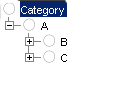
\includegraphics{PS/Treeexample4}
\caption{Tree 4}
\label{treeexample4}
\end{center}
\end{figure}
\end{itemize}
